\chapter{A Main Controller Board}

The Raspberry PI Pico is a powerful controller with a dual core, generous program and memory sizes and USB also included. The Pico is a small board that can be soldered to a mother PCB or connected just like a big IC. This chapter will present our main controller board which is just the controller along to a CAN bus interface, the non-volatile memory and the level shifters to accommodate our 5V interface level standard. Although there will be more different controller boards in the chapters to come, this basic building block is the generic heart and can be used for many other projects in the LCS system.

\section{Block Diagram}

The following schematic depicts the block diagram of our main controller. All of our schematics will start with a block diagram and the one or more parts of the overall schematic.

\begin{figure}[htbp]
    \centering
    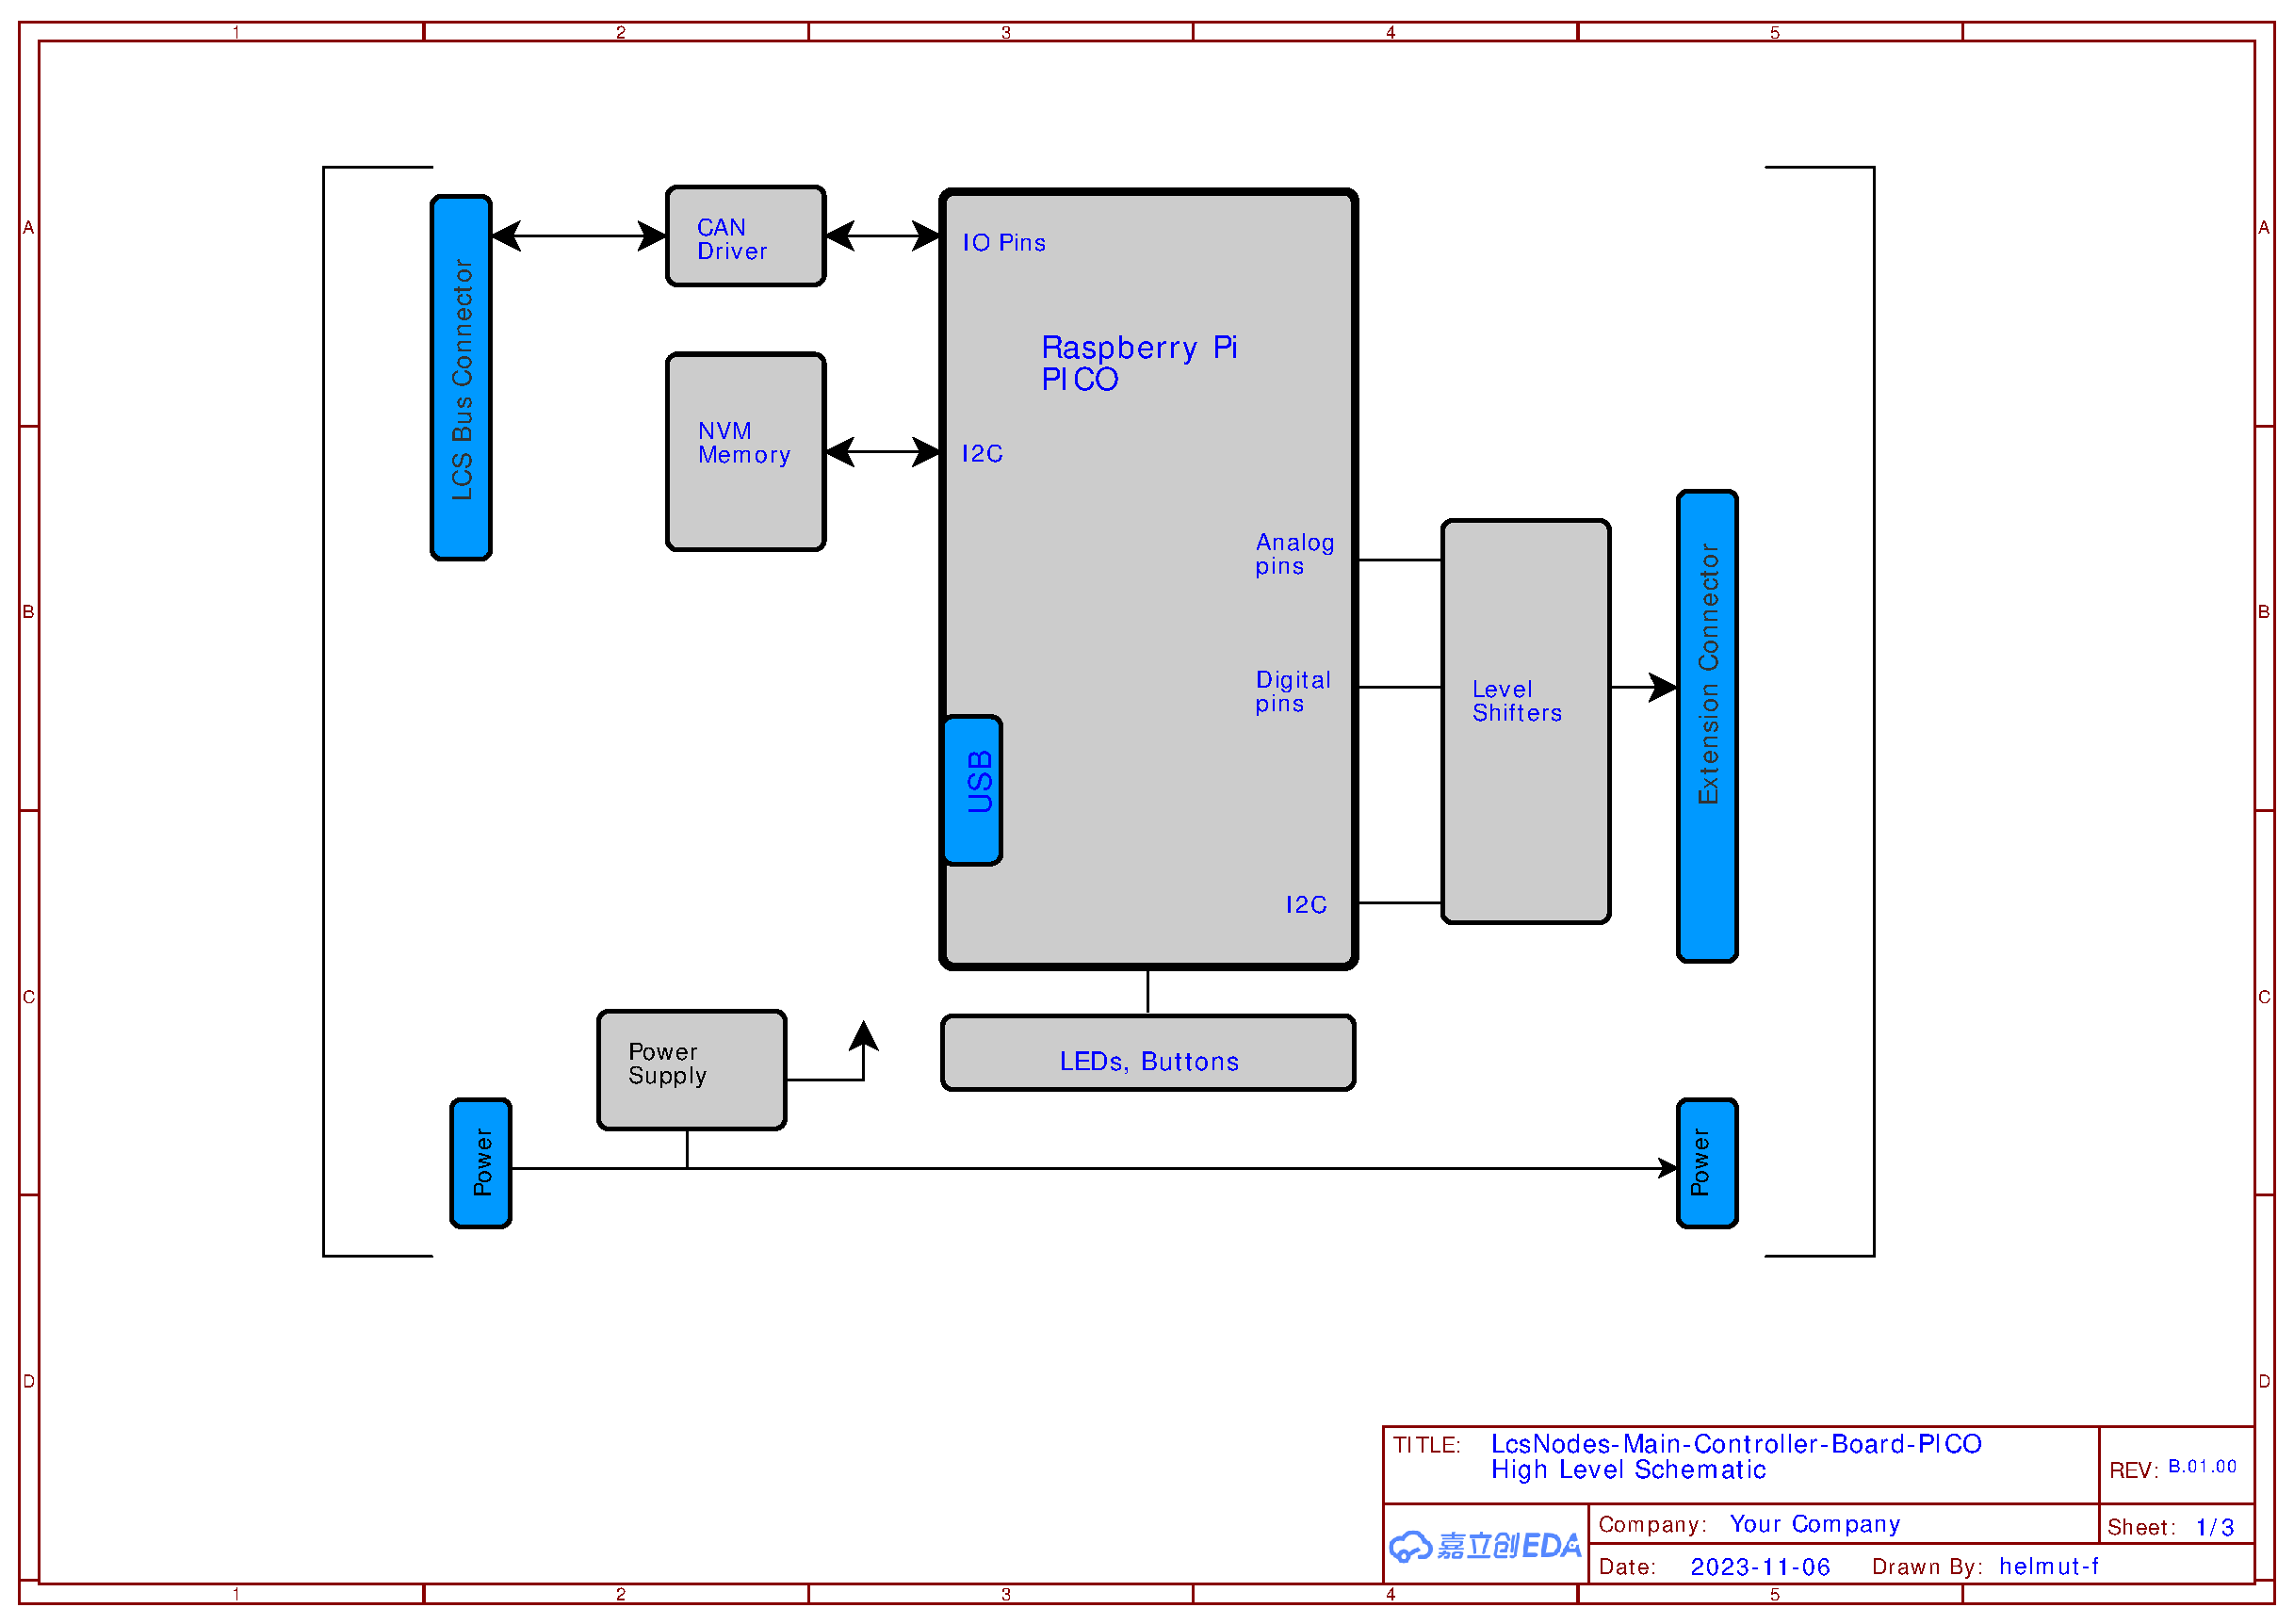
\includegraphics[page=1, width=0.8\textwidth]{./Schematics/Schematic_LcsNodes-Main-Controller-Board.pdf}
    \caption{Main LCS Controller Block Diagram}
    %\label{fig:schematic}
\end{figure}
\FloatBarrier

\section{Main Controller}

The first part of the schematics shows the PICO processor, LEDS, Button, CAN bus driver and NVM storage as well as the power supply with the optional power fail capability.

\begin{figure}[htbp]
    \centering
    \includegraphics[page=2, width=0.8\textwidth]{./Schematics/Schematic_LcsNodes-Main-Controller-Board.pdf}
    \caption{Main LCS Controller Controller Part}
    %\label{fig:schematic}
\end{figure}
\FloatBarrier

\section{Connectors and Level Shifters}

The second part depicts the connectors and the level shifters.

The ADC inputs also need a divider to map the incoming voltage range of 0 to 5V to 0 to 3V3. A simple resistor divider does the job.


??? talk about the mapping of PICO pins to extension connector pins. Should allow that function blocks such as SPI, UART, I2C, etc can be accessed.

\section{PICO Pin Mapping}

EXT             - pin 4

DIO 0,1         - 6,7

DIO 2,3         - 8,9

DIO 4,5         - 10,11

DIO 6,7         - 12,13

DIO 8,9         - 18,19

DIO 10,11       - 20,21

CAN             - 0,1

I2C NVM         - 2,3

I2C EXT         - 16,17

Ready Led       - 14

Activity Led    - 15



\begin{figure}[htbp]
    \centering
    \includegraphics[page=3, width=0.8\textwidth]{./Schematics/Schematic_LcsNodes-Main-Controller-Board.pdf}
    \caption{Main LCS Controller Connector and Level Shifters}
    %\label{fig:schematic}
\end{figure}
\FloatBarrier

\section{A Main Controller Board PCB for PICO}

And here is the PCB for the PICO based main controller. It is a 10cmx 12cm board. Note that there is quite some real estate allocated to the level shifters between 5V and 3V3. When most of the IO pins are used in a monolithic board design, these level shifters are perhaps not needed. Since our extension connectors standardizes on 5V for digital levels, we we need them for this board.

\begin{tikzpicture}[scale=0.9, transform shape]
    \draw[help lines, gray!50, dashed] (0,0) grid( 16,8);
    \node at (8,4) {picture};
\end{tikzpicture}
\FloatBarrier

\section{Summary}

By now we have a core library which can handle the basics of just about any node and we have a main controller board that will form the heart of many projects to come for the layout control system. However, while LCS boards will all run the same core library, there are still differences how for example the controller pins are assigned on the boards. It is very likely that new software versions and perhaps different processors and boards layouts will require that the core library is adapted to each processor / board combination. This is especially true for monolithic board designs, where there is a great freedom which pins to use for what. At this point, many projects found on the web will now start a symphony of "ifdefs" in their coding. The conditional compiles often reach up to the highest layers of the firmware programming. 

Perhaps there is a way to shield all these differences at a lower layer such that higher level libraries and firmware just refer to symbolic names for controller functions and pins. A mapping structure will translate between the symbolic names and the actual HW counterpart. This \textbf{controller dependent layer} will be the topic of the next chapter.

Just before we move on, what can be done with this board ?. It seems to be just a fancy wrapping around the controller chip. Well, first of all, it is a fully function node, capable of receiving CAN bus messages. It also features the library runtime storage and exports a variety of pins to the extension connector. During the development of the concepts and the runtime library this board served as the development platform. When designing a new node type, it is a great starting point to take care of the main controller part, allowing to concentrate fully on the node additional capabilities. We will pick up on this in later chapters when extensions are presented.    
